\scanpage{44}
Genre de la courbe de Fermat $C_n$ (qui est une courbe
\inserted{plane} \deleted{\unsure{projective}} lisse de degré $n$)
\[
g_n=\frac{(n-1)(n-2)}2
\]
Le genre est 0 ssi $n=1,2$, il est 1 ssi $n=3$.
Pour $n=4$ il est 3, pour $n=6$ il est 10,
pour $n=12$ il est $55\ldots$

\rule{3cm}{0.4pt}

Considérons le cas $n=2$
\[
C_2:\quad x^2+y^2+z^2=0
\]
comme carte triangulée pondérée elle est formée de $4.2=8$ triangles,
chaque type de sommet intervient 2 fois, avec degré
$4$ \inserted{$(2.2)$} en chaque sommet.
Sauf erreur, c'est l'\uline{octaèdre} \inserted{sphérique}, dont le groupe des
automorphismes orientés est bien \inserted{$\simeq\unsure{\mathfrak S_4|\mathbb G_4}$}
d'ordre 24, et peut s'écrire comme produit $\frac12$ direct de
$\unsure{\mathfrak S_3|\mathbb G_3}$ par $(\mathbb Z_2)^2$ !
\figure{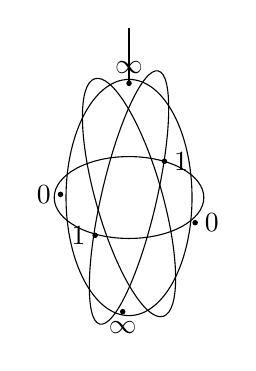
\begin{tikzpicture}[x=1cm,y=1cm]
\draw (0,0) ellipse (.8 and 1.5);
\draw (0,0) ellipse (.95 and .52);
\draw[rotate=-13] (0,0) ellipse (.35 and 1.65);
\draw[rotate=16] (0,0) ellipse (.42 and 1.57);
\draw (0,1.46)--(0,2.15);
\foreach \x/\y/\lab/\pos in {0/1.45/\infty/above,-.87/.04/0/left,.45/.46/1/right,.84/-.32/0/right,-.43/-.48/1/left,-.08/-1.45/\infty/below}{
\fill (\x,\y) circle (.035);\node[\pos] at (\x,\y) {$\lab$};}
\end{tikzpicture}}
% crop-candidate: scan 44
Divisant par les trois s-groupes $\mathbb F_2$ de
$\pi_2\simeq\mu_2^3/\mu_2$, on trouve les \inserted{3} revêtements
d'ordre 2 de $C_1:\simeq\mathbb P^1_{\mathbb Q}$ qui correspondent
au \deleted{dièdre} \inserted{monoèdre} \deleted{$\unsure{i=1}$}
(standard) et à ses transformés par $\unsure{\mathfrak S_3|\mathbb G_3}$.

\margin{\uline{NB} L'octaèdre est subdivision barycentrique du bi-èdre
(qui est autodual \unsure{\&|$*$} et a le type de ramification
\[
\begin{array}{ccc}2&2&2\\2&2&2\end{array}
\]
(cas particulier de celui du dièdre
\[
n\left\{\begin{matrix}2\\\vdots\\2\end{matrix}\right.\quad
\unsure{n}\left\{\begin{matrix}2\\\vdots\\2\end{matrix}\right.\quad
\begin{matrix}n\\n\end{matrix},\quad\text{pour }n=2),
\]
\unsure{ce qui} \uline{\unsure{entraîne|combinatoire}}, on le voit
de suite le rev. abélien universel
\inserted{\unsure{du monoèdre} \unsure{par} $\unsure{2}\unsure{\mathbin{-}}$}}
\figure{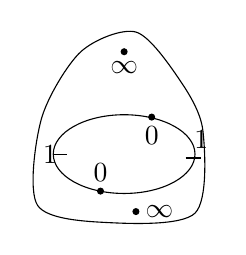
\begin{tikzpicture}[x=1cm,y=1cm]
\draw plot[smooth cycle] coordinates {(-1.1,-.65)(-1.05,.45)(-.55,1.3)(.15,1.55)(.7,.95)(1,.3)(.9,-.75)(-.2,-.87)};
\draw (0,0) ellipse (.9 and .5);
\fill (0,1.3) circle (.045) node[below] {$\infty$};
\fill (.15,-.73) circle (.045) node[right] {$\infty$};
\fill (.35,.47) circle (.045) node[below] {$0$};
\fill (-.3,-.47) circle (.045) node[above] {$0$};
\draw (-.9,0)--(-.73,0) node[left] {$1$};
\draw (.78,-.05)--(.98,-.05) node[above] {$1$};
\end{tikzpicture}}
% crop-candidate: scan 44
% The marginal note runs to and is physically clipped by the lower image edge.
% archive foliation: 43
